\chapter{The most exciting observable}
\label{ch:nedm-at-psi}

% \begin{center}
%   \emph{The chief forms of beauty are order and symmetry and definiteness, which the mathematical sciences demonstrate in a special degree.}\\
%   Aristotle
% \end{center}


% \begin{center}
%   \emph{Why are we here? Because of CP-symmetry violation.}\\
%   prof. Edward Hinds
% \end{center}

\begin{flushright}{\slshape    
  The chief forms of beauty are order and symmetry and definiteness,\\
  which the mathematical sciences demonstrate in a special degree.} \\ \medskip
--- Aristotle
\end{flushright}

\bigskip

\begin{flushright}{\slshape    
  Why are we here?\\
  Because of CP-symmetry violation.} \\ \medskip
--- prof. Edward Hinds
\end{flushright}

\bigskip

\section{Symmetries}

% Symmetry is the most fundamental form of beauty.

The essence of the classical physics are the three symmetries: with respect to the spatial translation (homogeneity of space), with respect to rotation (isotropy of space) and with respect to translation in time (homogeneity of time). As Noether showed, they correspond to the conservation laws of momentum, angular momentum and energy, respectively~\cite{Noether1918}. By saying a symmetry is conserved, we understand that no physical system becomes any different by \emph{only} having been moved in space, rotated, or looked at later.

These are continuous symmetries. No less fundamental is the triad of symmetries with respect to discrete transformations: $P$, parity transformation, mirroring the spatial dimensions; $T$, time reversal, flipping the arrow of the time; and $C$, charge conjugation, flipping \emph{all} charges of particles. One would expect a beautiful universe to work exactly the same in the mirror, or with matter swapped with anti-matter.

Discrete symmetries can be combined. So $CP$ means a symmetry after flipping the charges \emph{and} mirroring the space. The combined $CPT$-symmetry is obeyed by any Lorentz invariant local quantum field theory with a Hermitian Hamiltonian~\cite{Sachs1987}. It scares a humble experimental physicist to think of a theory which would not fulfill this.

Yet, in a perfectly symmetric universe after the Big Bang an equal amount of matter and anti-matter would be created and they would perfectly annihilate. There would not be us.
In 1967 Andrei Sakharov
\marginpar{Andrei Sakharov, pacifist and human-rights activist, was awarded the 1975 Nobel Piece Price, called ``a spokesman for the conscience of mankind''.}
has formulated that a necessary condition for that not to happen, for there to be a bit of matter left over, is a violation of the $CP$-symmetry~\cite{0038-5670-34-5-A08}.

Physicist have now long accepted violations of the fundamental symmetries.
The first shock came in 1956 with Chien-Shiung Wu's discovery of a $P$ violation in beta decay of cobalt-60~\cite{PhysRev.105.1413}. Shortly thereafter, in 1964, the discovery of a $CP$ violation in $K^0_L \rightarrow \pi^+ \pi^-$ decay left the physics world stunned again~\cite{PhysRevLett.13.138}. Now both are explained in the scope of the Standard Model of particle physics. In the Model the $CP$-violation appears in the weak sector as a complex phase in the Cabbibo--Kobayashi--Maskawa matrix---the matrix that mixes the mass- and interaction-eigenstates of quarks~\cite{doi:10.1143/PTP.49.652}.

$CP$ violation also appears in the strong sector of the Standard Models quantum chromodynamics, as an additional term parametrised by $\theta_\text{QCD}$. Yet, no $CP$ violation in the strong sector has been indicated by the experiment, limiting the expected $\mathcal{O}(1)$ parameter $\theta_\text{QCD}$ to be smaller than \num{e-10}~\cite{PDG2016}. A puzzle in itself, it is referred to as the strong $CP$ problem.

All together, the degree of $CP$-symmetry violation in the Standard Model is not enough to explain the Universe we observe. The observed matter--anti-matter asymmetry is around \num{e-10}, while only \num{e-18} can be attributed to the Model~\cite{Riotto1999}. Despite the tremendous success of the Standard Model, we know it is not the full picture. We \emph{know} that the $CP$-symmetry is violated somewhere still, but do not know neither where or how~\cite{Pospelov2005}. Naturally, we want to find out. 

Many theories beyond the Standard Model have been proposed that offer to solve this, among others, problem. A very popular idea is to introduce additional particles around the scale of weak interactions (several-hundred GeV), as, for example, supersymmetry does \note{cite}. Those theories typically introduce additional mechanisms of $CP$-violation, which provide an opportunity to test their prediction~\cite{Ellis1989}.



\section{The neutron electric dipole moment}

Excellent probes for these theories are electric dipole moments (EDMs)~\cite{Pospelov2005}. An EDM is a $T$-violating, so assuming $CPT$ conservation, also $CP$-violating observable. In a non-relativistic case of a particle in an electric and magnetic field, with the magnetic and electric moments $\mu$ and $d$, the hamiltonian is:
\begin{equation}
  H = - \mu \, \bm{B} \cdot \frac{\bm{S}}{S} - d \, \bm{E} \cdot \frac{\bm{S}}{S} \ .
\end{equation}
For a spin $S = \frac{1}{2}$ particle:
\begin{equation}
  H = - \tfrac{1}{2} \left( \mu \, \bm{B} + d \, \bm{E} \right ) \cdot \bm{S} \ .
\end{equation}
Vectors, like $\bm{E}$, are $P$-odd, while pseudovectors, $\bm{B}$ and $\bm{S}$, are $P$-even. The hamiltonian as whole is $P$-odd:
\begin{equation}
  H_P = - \tfrac{1}{2} \left( \mu \, \bm{B} - d \, \bm{E} \right ) \cdot \bm{S} \neq H \ .
\end{equation}
Under the time symmetry the spin is reversed and so is the magnetic field, rendering the hamiltonian $T$-odd:
\marginpar{Magnetic field is produced either by magnetic moments, which flip under $T$ together with spins, or by a movement of charges, which also is reversed under $T$.}
\begin{equation}
  H_T = H_{CP} = + \tfrac{1}{2} \left( - \mu \, \bm{B} + d \, \bm{E} \right ) \cdot \bm{S} = - \tfrac{1}{2} \left( \mu \, \bm{B} - d \, \bm{E} \right ) \cdot \bm{S} \neq H \ .
\end{equation}
Note how in both cases setting $d = 0$ restores the symmetry.

EDMs are measured mainly in three kinds of systems. Beams of cold paramagnetic molecules, like YbF, provide a great sensitivity to the EDM of the electron~\cite{Hudson2011}. Measurements of vapours of diamagnetic atoms, notably $^{199}$Hg~\cite{PhysRevLett.116.161601}, are the most sensitive EDM measurements. Finally, the electric dipole moment of a free neutron, nEDM, which is the topic of this chapter.

While the Standard Model predicts the nEDM to be below \SI{e-30}{\elementarycharge\centi\meter}, its extensions foresee it to be \SIrange[range-phrase=--,range-units=single]{e-29}{e-22}{\elementarycharge\centi\meter}. Experimental exploration of this range provides an opportunity to validate, or falsify, those theoretical models. \note{cite for the lower range}. Also, the neutron EDM, provides the most sensitive handle on measurement of the on $\theta_\text{QCD}$, parametrising the strong $CP$ problem.



\section{Measurements of the nEDM}

\begin{figure}
  \centering
  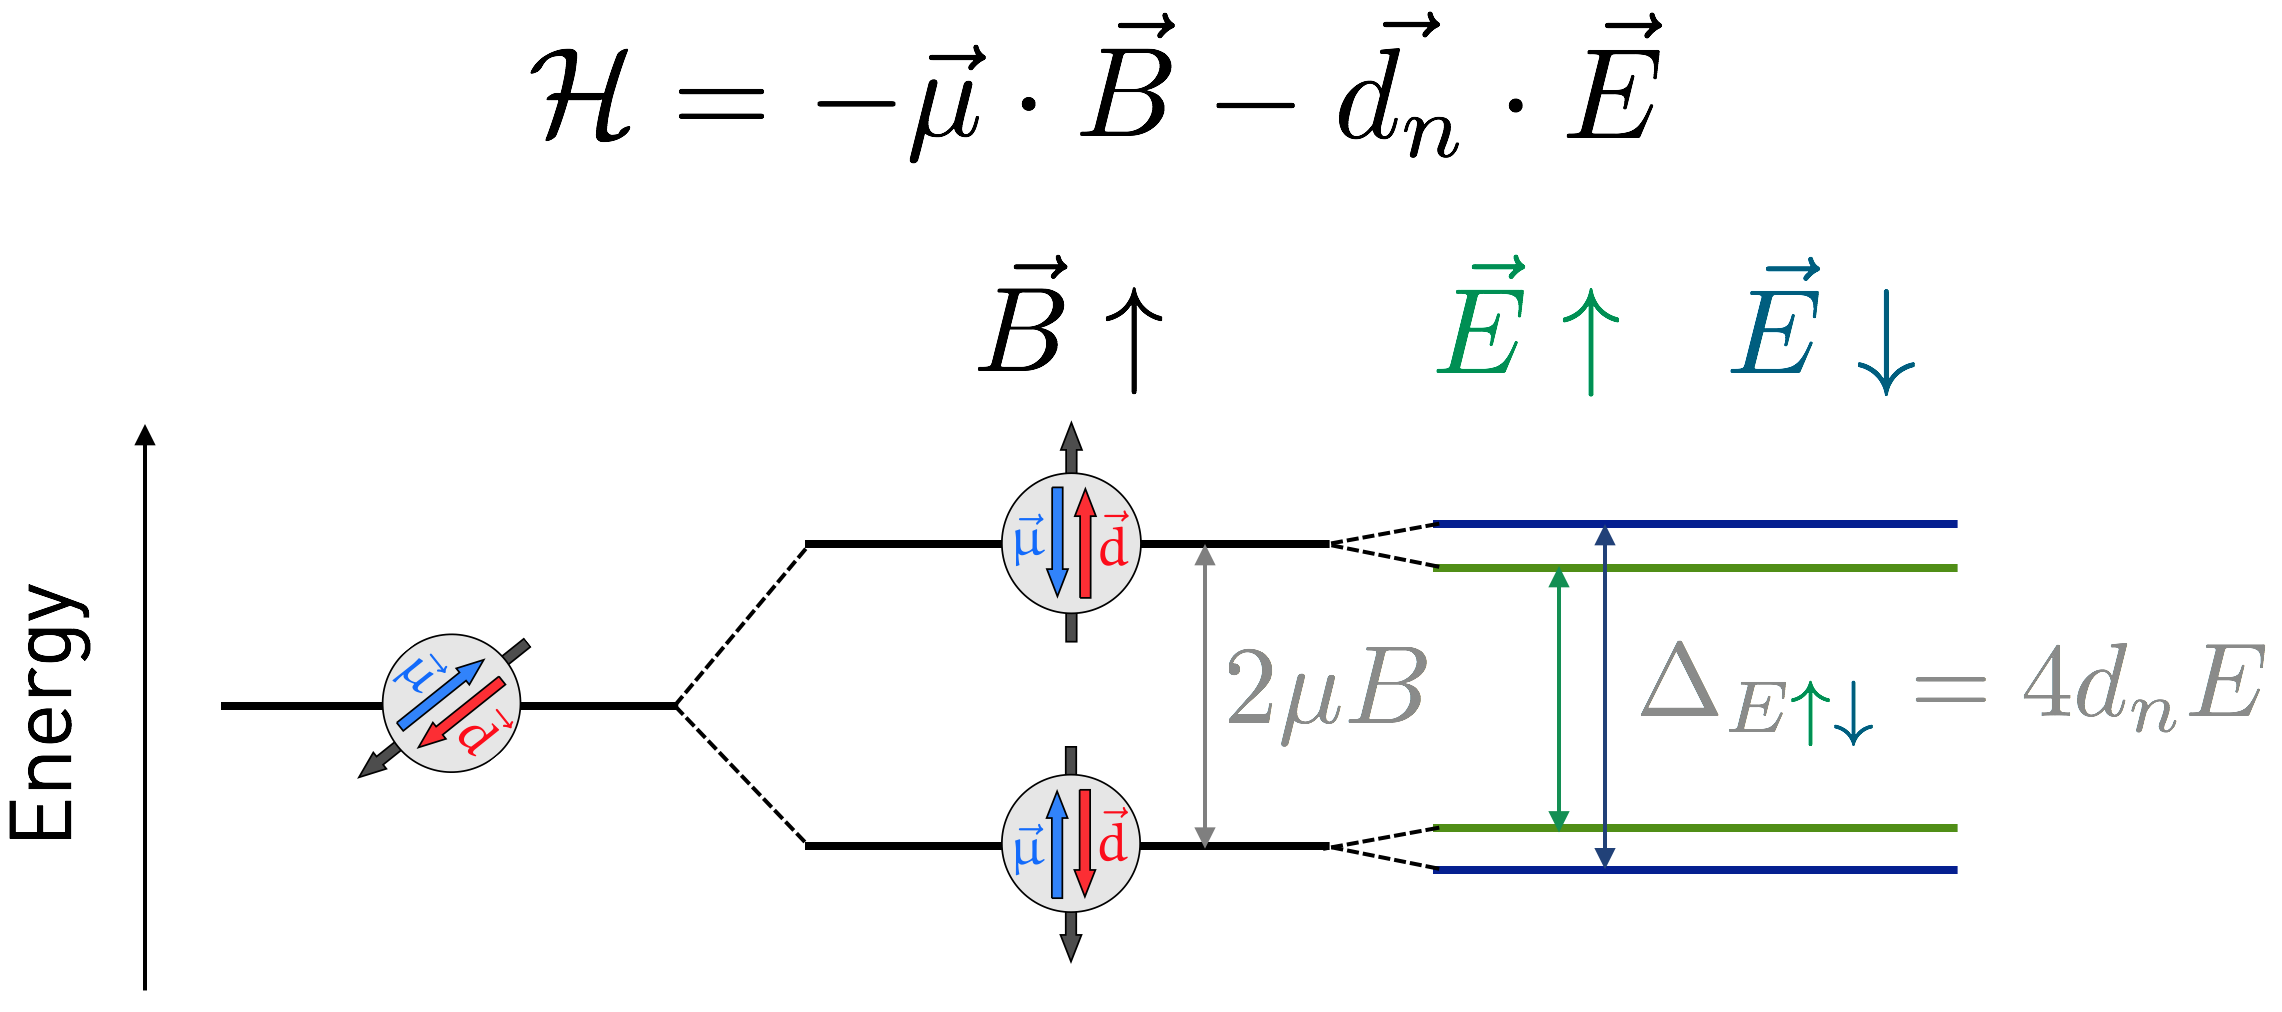
\includegraphics[width=\linewidth]{gfx/nEDMatPSI/measurement_principle.png}
  \caption{The energy states of a neutron in a combination of a magnetic and electric fields. The hamiltonian is $H = - \frac{1}{2} \left( \mu_\text{n} \, \bm{B} + d_\text{n} \, \bm{E} \right ) \cdot \bm{S}$. The first term causes the first splitting, $2\mu_\text{n} B$ large. The second term increases or decreases, for the electric field parallel and anti-parallel to the magnetic one respectively, the splitting by $2 d_\text{n} E$.}
  \label{fig:nEDM_measurement_principle}
\end{figure}

Already in 1949, before Wu's discovery of $P$-violation in the weak sector, Purcell and Ramsey performed a measurement to test $P$-violation in the strong sector using the nEDM as the probe~\cite{PhysRev.108.120}. They got a zero-consistent result $d_n = (-0.1 \pm 2.4) \times 10^{-20}\,\si{\elementarycharge\centi\meter}$.

As shown in Fig.\,\ref{fig:nEDM_measurement_principle} a neutron in a magnetic field $B$ has two energy states, separated by $2 \mu_\text{n} B$. The apparatus of Purcell and Ramsey could measure this separation, as a frequency, very precisely. Additionally to the magnetic field there was an electric one, either parallel or antiparallel to it. If there had been an nEDM, the energy separation would have increased in one configuration and decreased in the other. The difference between the energy separations measured in the two field configurations is proportional to the nEDM $d_\text{n}$.

\begin{figure}
  \centering
  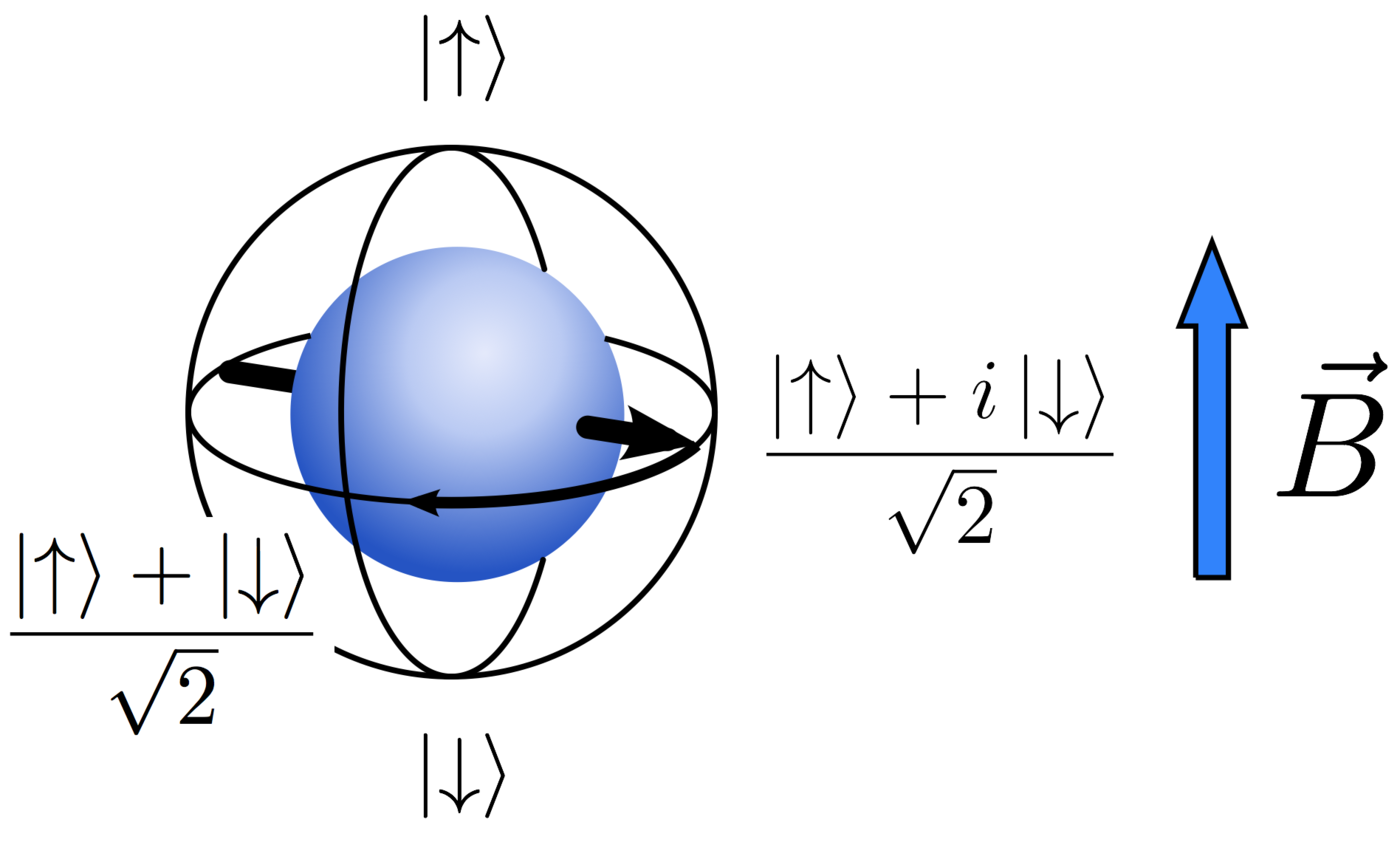
\includegraphics[width=.6\linewidth]{gfx/nEDMatPSI/bloch_sphere.png}
  \caption{A spin $\tfrac{1}{2}$ particle in a magnetic field on a Bloch sphere. The poles correspond to the pure spin-up and spin-down states. On the equator lie the states with an equal contribution of the two and the longitude corresponding to the quantum phase.}
  \label{fig:nEDM_bloch_sphere}
\end{figure}

To measure the energy separation between the two spin states they used what is now called the Ramsey method of separated oscillatory fields. In order to explain it, let us first consider a neutron in a magnetic field, as pictured in Fig.\,\ref{fig:nEDM_bloch_sphere}. The neutron's spin is depicted there on the Bloch sphere, where the poles correspond to the pure spin-up and spin-down states. On the equator lie the states with equal content of the two, the longitude marking the quantum phase. When the spin state is not vertical the interaction between the magnetic moment and the magnetic field exerts a torque that sets it into rotational motion, called Larmor precession.

\begin{SCfigure}
  \centering
  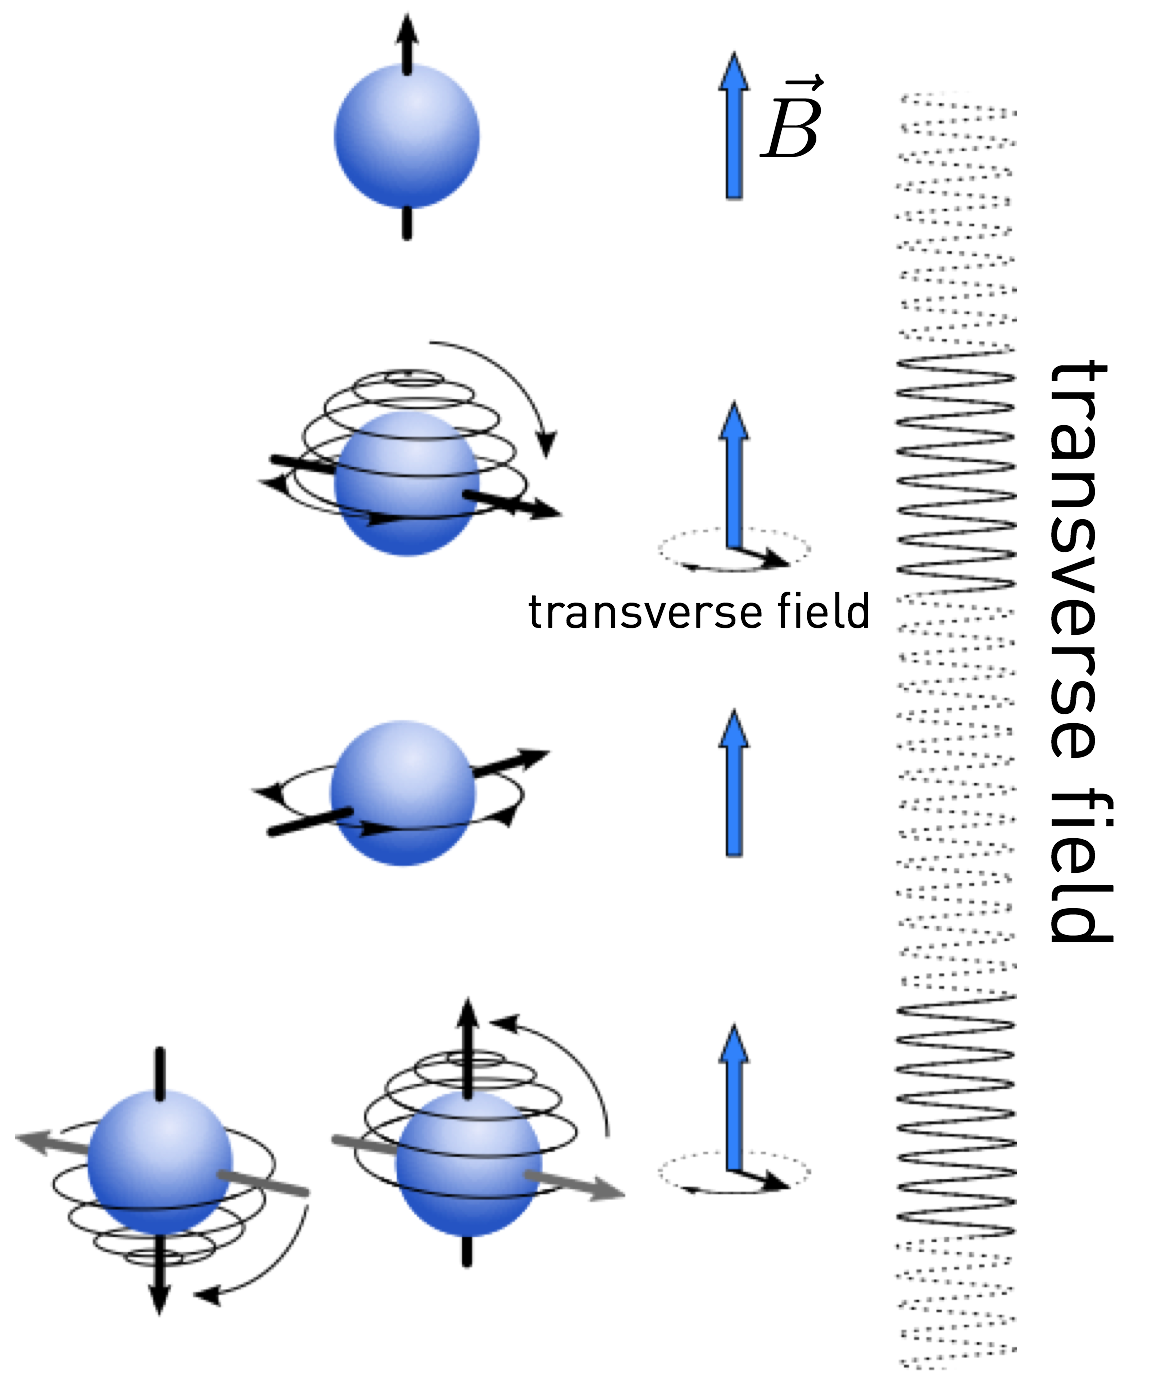
\includegraphics[width=.6\linewidth]{gfx/nEDMatPSI/Ramsey_principle.png}
  \caption{The principle of the Ramsey method, explained with the spin on the Bloch sphere. A polarised spin ensemble is in a magnetic field. A pulse of an oscillating transverse field flips the polarisation into the horizontal plane. The spin is allowed to freely precess in the field. Then, a second pulse of a transverse field is applied, in phase with the first one. The direction of the polarisation's flip depends on the relative phase between the spin and the transverse field.}
  \label{fig:nEDM_Ramsey_principle}
\end{SCfigure}

\begin{figure}
  \centering
  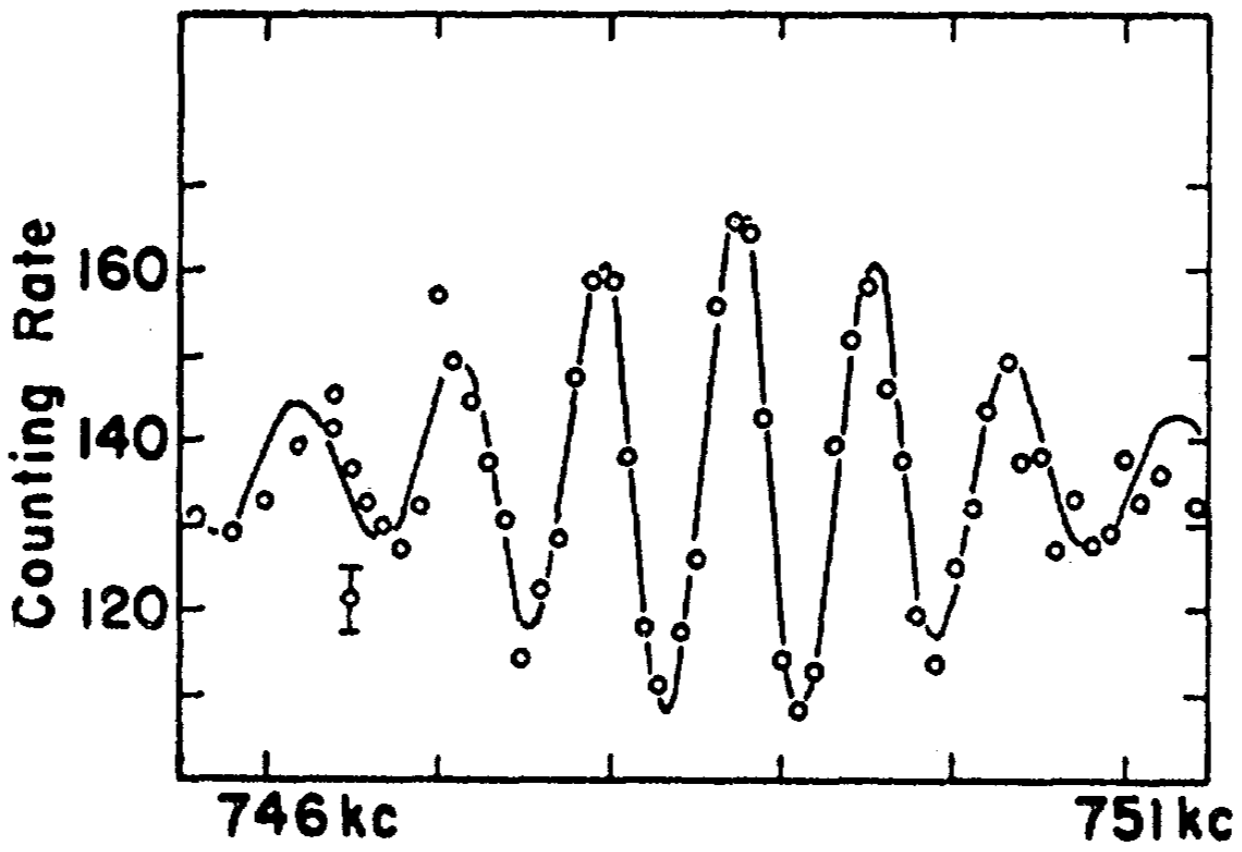
\includegraphics[width=.6\linewidth]{gfx/introduction/Ramsey_original_resonance.png}
  \caption{The original resonance curve measured by Ramsey~\cite{PhysRev.108.120}. The counting rate versus the frequency of the generator powering the spin-flipping coils. The fringes are due the interference between the precessing spins and the transverse field. Their width is the inverse duration of the free precession. The envelope arises, as at a large detuning the spins were not flipped into the horizontal plane anymore.}
  \label{fig:nEDM_Ramsey_original_curve}
\end{figure}

In the experiment the neutron beam passed through a polariser, a region with a magnetic and electric fields, and landed after an analyser on a neutron counter. At the beginning and the end of the region with the fields there were coils producing an oscillating magnetic field in the direction perpendicular to the main field. The spin evolution between the two coils is depicted in Fig.\,\ref{fig:nEDM_Ramsey_principle}. When a neutron precessing in a magnetic field feels an additional oscillating field, transverse to the main one and of frequency close to the one of its precession, its spin undergoes a nutation---the precession plane moves along the main field (North or South on the Bloch sphere). The direction is determined by the relative phase between the spin's precession and the transverse oscillating field. The length of the coils was set to flip the neutrons' spins by $\pi/2$, so that after having passed the first coil they were precessing on the Bloch sphere's equator. The direction of the nutation in the second coil, and with it the probability of passing the analyser, depended on the relative phase between the precession and the transverse field. A slight change in the frequency of the generator powering the coils caused a considerable change in the phase difference that builded up while the neutrons flew precessing between the coils. Scanning the frequency of the generator and monitoring the counting rate produced a resonance curve (Fig.\,\ref{fig:nEDM_Ramsey_original_curve}). The middle of the central fringe is the resonance frequency corresponding to the transition energy between spin-up and spin-down states.

\begin{figure}
  \centering
  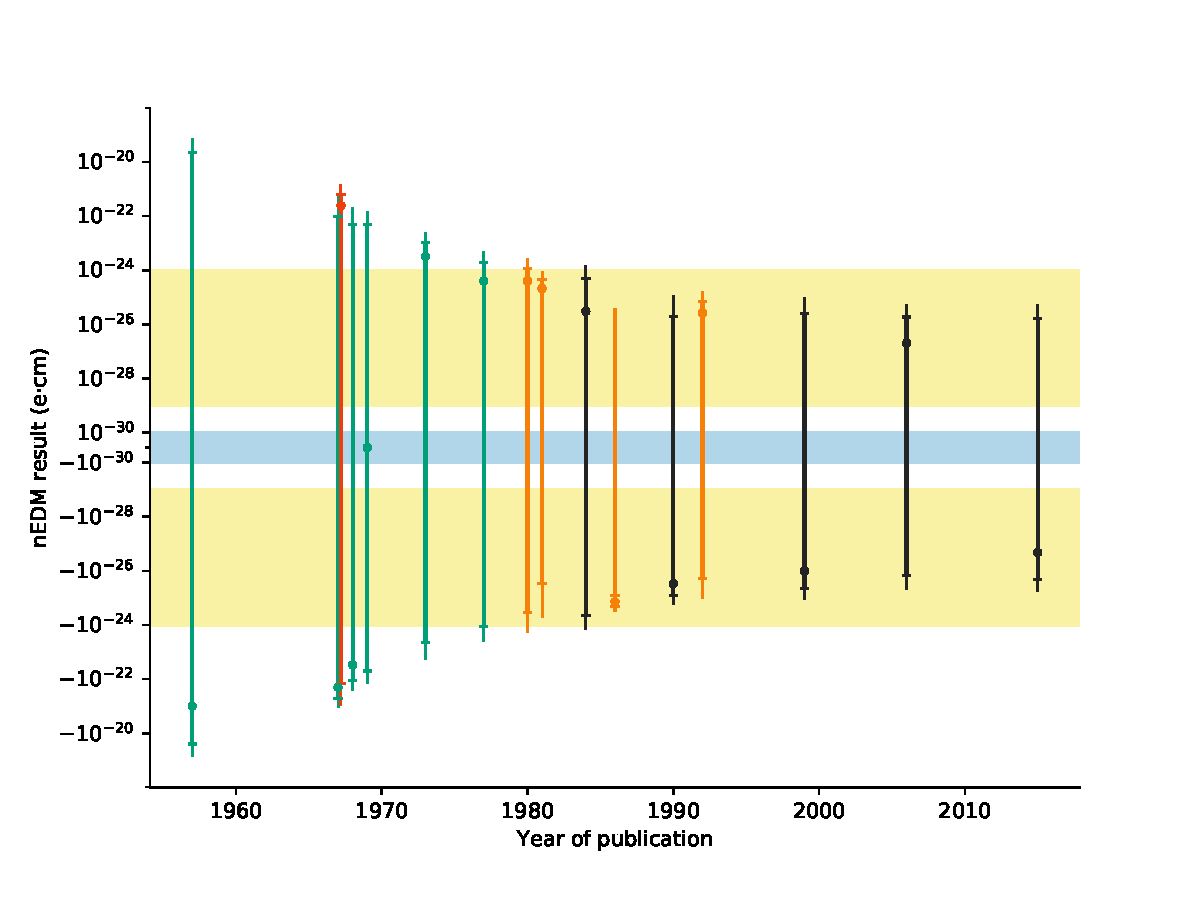
\includegraphics[width=\linewidth]{gfx/introduction/edm_limits.pdf}
  \caption{The history of the neutron electric dipole moment measurements. For each published result the vertical line corresponds to the $3\upsigma$ allowed region, horizontal bars depict the $1\upsigma$ one. Dots are located at the central values of the measurements. The vertical scale is a combination of two logarithmic ones---one for each sign of nEDM. The region of the Standard Model's prediction is depicted in blue, the one of the proposed Model's extensions in yellow. The red line indicates a result obtained from a neutron scattering experiment. The sources are, in chronological order:~\cite{PhysRev.108.120,PhysRevLett.19.381,PhysRevLett.19.384,PhysRev.170.1200,PhysRev.179.1285,PhysRevD.7.3147,PhysRevD.15.9,ALTAREV1980269,ALTAREV198113,altarev1986search,ALTAREV1992242,PENDLEBURY1984327,SMITH1990191,PhysRevLett.82.904,PhysRevLett.97.131801}}
  \label{fig:nEDM_limits_history}
\end{figure}

\marginpar{In the LNPI measurements slightly differ from Ramsey's technique by using an adiabatic transition in inhomogeneous magnetic field instead of spin-flips was used to account for different storage times of individual neutrons, which freely traveled through the bottle.}
The community uses this technique to measure the nEDM until this day. Figure\,\ref{fig:nEDM_limits_history} summarises these efforts of ever-increasing sensitivity. The measurements were done using a beam of cold neutrons until 1970s (marked in green).
In 1980 in the Leningrad Nuclear Physics Institute (LNPI, former USSR) the first measurement was performed with the neurons being stored in a bottle, rather than on a beam~\cite{ALTAREV1980269}. Neutrons with kinetic energies below approximately \SI{100}{\nano\electronvolt} (referred to as ultracold) are storable in some materials, on which they undergo a total internal reflection~\cite{UCNbook}. This technique greatly improved the time of the free precession, and thereby the sensitivity. The measurements in LNPI continued (orange) and in 1984 were joined by an international effort in the Institute Laue-Langevin in France (black).

In 2007 a new effort has begun in the Paul Scherrer Institute (PSI) in Villigen, Switzerland. The experiment collected data over the years 2015--17 and at the time of writing the result was still being evaluated. The author had the honor to be part of this venture, which we will take a closer look at in the next chapter.

The rest of the work focuses on two aspects closely related to all nEDM measurements: stabilisation of the magnetic field and exotic physics that can be explored with those highly sensitive experiments.



\section{Magnetic stability}
The quality of the magnetic field is the main challenge in the measurements of nEDM. Recall the principle of the measurement, as depicted in Fig.\,\ref{fig:nEDM_measurement_principle}. $d_\text{n}$ is proportional to the difference in measured energy separations between the field configurations. Let us ask ourselves the following question: how big is a change in the magnetic field that causes a comparable change in the separation of the states?

The current limit is around $|d_\text{n}| < \SI{e-26}{\elementarycharge\centi\meter}$~\cite{PhysRevLett.97.131801}. This corresponds to an energy
\begin{equation}
  \Delta_{E\uparrow\downarrow} = 4 d_\text{n} E = \SI{4e-26}{\elementarycharge\centi\meter} \ \frac{ \SI{132}{\kilo\volt} }{ \SI{12}{\centi\meter} } = \SI{4.4e-22}{\electronvolt} \ .
\end{equation}
With the neutron magnetic dipole moment
\begin{equation}
  \mu_\text{n} = \SI{-9.7e-27}{\joule\per\tesla} = \SI{-6e-8}{\electronvolt\per\tesla} \ ,
\end{equation}
the size of a change in magnetic field corresponding to this energy is
\begin{equation}
  \frac{ \Delta_{E\uparrow\downarrow} }{2 \mu_n} = \SI{3.7e-15}{\tesla} = \SI{3.7}{\femto\tesla} \ .
\end{equation}
This is about the strength of the magnetic field of a car passing several kilometers away. \note{Some logic, what it means.}
% Even in the most quiet of nights the magnetic field at the experimental site was not more stable than about a nanotesla, and during a day the variations reached tens of microteslas.

The nEDM experiments continue to set the world's standard in terms of stabilising and measuring magnetic fields~\cite{GREEN1998381,1748-0221-10-12-P12003,Groeger2005,Baker2014}. When it comes to stabilisation, a newcomer in the field is an active magnetic field stabilisation system. It was first used in the nEDM measurement at PSI, increasing the field stability by a factor of 5--50~\cite{Afach2014}. The second part of this work is dedicated to research in this area. It starts with technical developments related to maintaining the PSI's system over the course of three years. Then a novel method of designing coils is introduced, which makes active stabilisation systems more compact and effective. It is followed by a presentation of a system constructed at the ETH Zürich, intended as a small-scale prototype of a next-generation system for the nEDM measurement in PSI. Finally we describe a survey of the magnetic field in PSI's experimental area, a part of research on the magnetic field compensation there.


\section{Exotic physics}
\note{Really exotic? This sounds somewhat pejorative.}

The high sensitivity of the nEDM experiments invites them to additonally probe non-standard physics. For example a search for a short range spin-dependent interaction mediated by axions or axion-like particles~\cite{Afach2015Exotic}. Or testing the Lorentz invariance by looking for variations arising due to the Earth spinning in an nonisotropic Universe~\cite{Altarev2009,ALTAREV20112365}. Another idea is to restore the global $P$-symmetry by introducing mirror particles. Neutron to mirror-neutron oscillations could be detected with an nEDM apparatus~\cite{PhysRevD.80.032003}.

The author was proud to take part in starting a new area of non-standard physics searches with nEDM experiments. One of the candidates for dark matter are axions, extremely light particles generalising the idea of promoting the $\theta_\text{QCD}$ parameter into a field~\cite{PhysRevLett.38.1440}. An axion dark matter would form a coherently, very slowly (as slowly as days) oscillating field. This would induce coherent variations in the measured values of nEDM. A search for such variations is discussed in the part three.